\begin{frame}
 \frametitle{L'implémentation}

\begin{itemize}
 \item Langage Java
 \item Utilise des fichiers .data en entrée
 \item Utilisation de la librairie Weka pour l'implémentation de C4.5
\end{itemize}
3 exécutables : 
\begin{itemize}
 \item 2 en ligne de commande : 
    \begin{itemize}
      \item 1 pour classer un fichier .data avec C4.5 ou Naivebayes
      \item 1 pour classer plusieurs fichiers .data. Retourne un tableau LaTeX.
    \end{itemize}
  \item 1 interface graphique.
\end{itemize}

\end{frame}

 \begin{frame}%[plain]
%\begin{agrandirmarges}{1cm}{1cm}
 \begin{center}

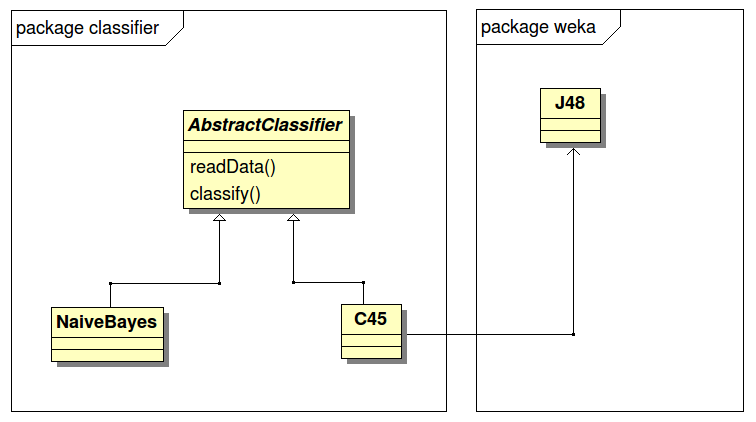
\includegraphics[width=320px]{classDiagram.png}
\end{center}

%\end{agrandirmarges}


\end{frame} 